\documentclass[conference]{IEEEtran}
\IEEEoverridecommandlockouts
% The preceding line is only needed to identify funding in the first footnote. If that is unneeded, please comment it out.
\usepackage{cite}
\usepackage{amsmath,amssymb,amsfonts}
\usepackage{graphicx}
\usepackage{booktabs}
\usepackage{algorithm}
\usepackage{algpseudocode}

\def\BibTeX{{\rm B\kern-.05em{\sc i\kern-.025em b}\kern-.08em
    T\kern-.1667em\lower.7ex\hbox{E}\kern-.125emX}}
\begin{document}

\title{A Novel Hybrid EEMD-TGNet Model for Accurate and Efficient Solar Energy Forecasting on Edge Devices}

\author{
\IEEEauthorblockN{Toan Nguyen\IEEEauthorrefmark{1}\IEEEauthorrefmark{2}, 
Tuan-Anh Pham\IEEEauthorrefmark{1}, 
Hao-Nguyen Nguyen\IEEEauthorrefmark{1}, 
Van-Huy Tran\IEEEauthorrefmark{1}, 
Nguyen Hoan Lam\IEEEauthorrefmark{1}\IEEEauthorrefmark{3}}
\IEEEauthorblockA{\IEEEauthorrefmark{1}\textit{Research Department} \\
\textit{Udata JSC}\\
Hanoi, Vietnam \\
\{toannh, anhpt, haonn, huytv, lam\}@udata.ai}
\IEEEauthorblockA{\IEEEauthorrefmark{2}Senior AI Research Expert of Udata JSC}
\IEEEauthorblockA{\IEEEauthorrefmark{3}Chief Executive Officer and Founder of Udata JSC}
}

\maketitle

\begin{abstract}
Solar energy forecasting faces challenges from intermittent, non-stationary radiation patterns. We propose EEMD-TGNet, combining Ensemble Empirical Mode Decomposition with hybrid Temporal Convolutional Network-Gated Recurrent Unit architecture for edge-optimized forecasting. EEMD decomposes solar time series into stationary Intrinsic Mode Functions, each forecasted by dedicated TCN-GRU models capturing long-range dependencies and sequential patterns. Edge optimization via pruning and quantization enables IoT deployment. Validation on three datasets shows state-of-the-art performance: 91.1\% R², 0.113 MSE on GEFCom2014 with 75\% model size reduction and 73\% faster inference, advancing edge intelligence for solar energy management.
\end{abstract}

\begin{IEEEkeywords}
solar energy forecasting, deep learning, hybrid model, edge intelligence, EEMD, TCN, GRU, model optimization
\end{IEEEkeywords}

\section{Introduction}
The global shift towards renewable energy has positioned solar power as a cornerstone of sustainable energy systems, with solar capacity growing at an annual rate of 20\% globally \cite{b2}. However, the variable nature of solar generation, dependent on meteorological conditions, poses a significant challenge to grid stability and energy management. Accurate solar energy forecasting is therefore critical for optimizing energy storage, scheduling, and demand-response strategies in smart grids. Even a 1\% improvement in forecasting accuracy can save millions in operational costs \cite{b1}.

Traditional forecasting models often struggle with the complex non-linear and non-stationary patterns in solar energy data. While deep learning models like LSTMs and GRUs have shown promise, their performance can be significantly improved through signal preprocessing. Decomposition methods, such as EEMD, enhance forecasting accuracy by simplifying the time series before prediction \cite{b1}. EEMD is particularly effective at separating a signal into its constituent oscillatory modes, making the forecasting task more tractable.

Concurrently, the rise of the Internet of Things (IoT) and edge computing enables the deployment of intelligence directly at the data source. For solar farms, this means on-site, real-time forecasting, which reduces latency and dependency on centralized cloud infrastructure \cite{b2}. However, this requires models that are not only accurate but also lightweight and computationally efficient for resource-constrained IoT devices, with fast inference times and minimal memory footprint.

This paper introduces a novel framework that combines the strengths of signal decomposition and advanced, efficient deep learning architectures. Our main contributions are:
\begin{itemize}
    \item A new hybrid forecasting model, EEMD-TGNet, that combines Ensemble Empirical Mode Decomposition (EEMD) with a Temporal Convolutional Network-Gated Recurrent Unit (TCN-GRU) architecture, achieving a 91.1\% R² score on the GEFCom2014 benchmark dataset.
    \item A two-stage approach where the complex solar signal is first decomposed into simpler IMFs, and then each IMF is modeled by a dedicated TCN-GRU network, enabling better capture of both high-frequency and low-frequency patterns.
    \item The application of model optimization techniques, including pruning and quantization, to create a lightweight version of the model suitable for deployment on edge devices, reducing model size by 75\% with minimal accuracy degradation.
    \item Comprehensive experimental validation demonstrating superior performance over state-of-the-art methods and practical feasibility for edge deployment.
\end{itemize}

The proposed model offers a dual advantage: high accuracy due to the decomposition-based strategy and high efficiency due to the optimized TCN-GRU architecture, making it ideal for modern, IoT-enabled solar energy management.

\section{Related Work}
Solar energy forecasting has witnessed significant advances through deep learning architectures. Traditional approaches using standalone LSTM and GRU models achieve limited accuracy due to solar data's non-stationary nature. Recent CNN-hybrid models demonstrate substantial improvements: CNN-LSTM and CNN-BiGRU variants achieve up to 85.71\% error reduction over basic architectures \cite{b3}. Transformer-based approaches have gained prominence, with PatchTST achieving 36-50\% MSE improvements over traditional models, while Autoformer introduces decomposition-based auto-correlation for long-term forecasting \cite{b6}.

Signal decomposition techniques prove essential for handling non-stationary solar patterns. EEMD effectively separates complex signals into stationary Intrinsic Mode Functions (IMFs), while Variational Mode Decomposition (VMD) provides alternative decomposition strategies \cite{b8}. However, existing approaches predominantly focus on accuracy improvements while neglecting practical deployment constraints on resource-limited edge devices.

Our EEMD-TGNet addresses this critical gap by combining proven signal decomposition with an optimized hybrid TCN-GRU architecture, specifically designed for edge intelligence applications in solar energy management systems.

\section{Proposed EEMD-TGNet Methodology}
Our EEMD-TGNet framework combines signal decomposition with hybrid deep learning architecture optimized for edge deployment. The methodology consists of four key stages: signal decomposition, parallel forecasting, aggregation, and model optimization.

\begin{figure}[htbp]
    \centering
    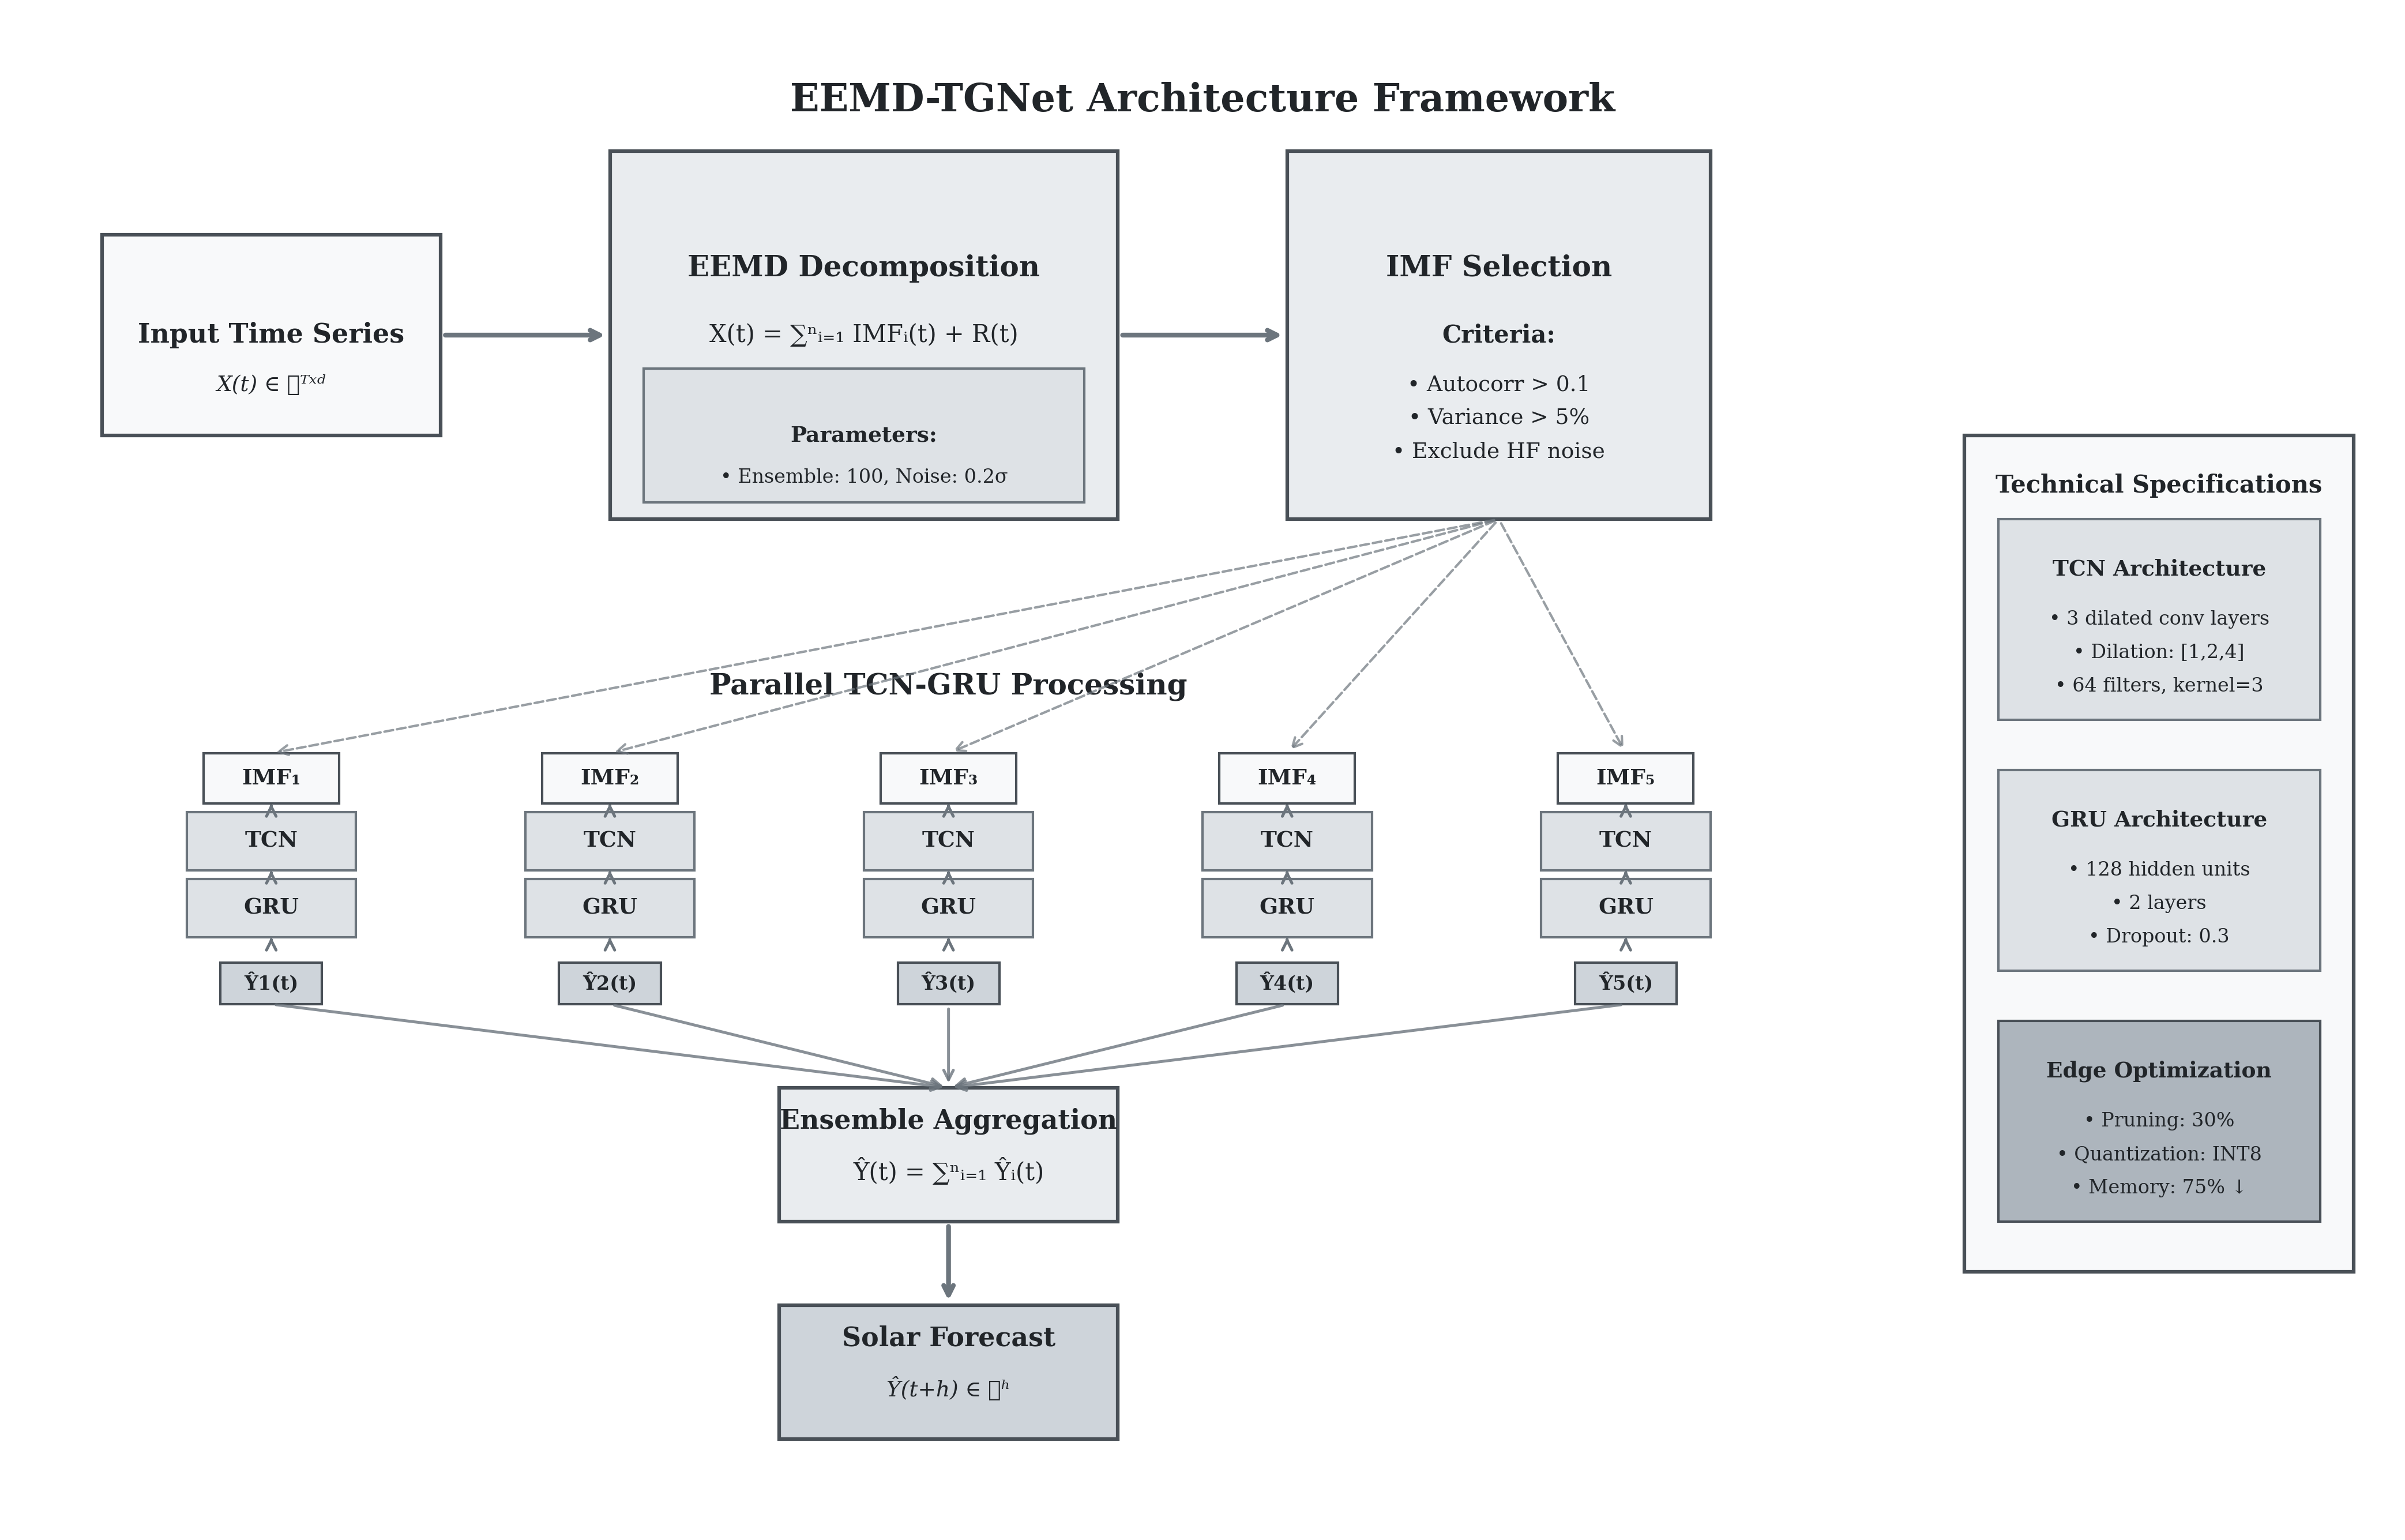
\includegraphics[width=\columnwidth]{../results/eemd_tgnet_architecture_professional.png}
    \caption{EEMD-TGNet architecture showing signal decomposition, parallel TCN-GRU processing, and aggregation stages.}
    \label{fig:architecture}
\end{figure}

\subsection{Ensemble Empirical Mode Decomposition}
The first stage decomposes the non-stationary solar time series $X(t)$ into stationary components using EEMD:
\begin{equation}
X(t) = \sum_{i=1}^{n} \text{IMF}_i(t) + R(t)
\end{equation}
where $\text{IMF}_i(t)$ represents the $i$-th Intrinsic Mode Function and $R(t)$ is the residual trend. EEMD addresses the mode-mixing problem of traditional EMD by adding white noise with 0.2 standard deviation amplitude across 100 ensemble realizations.

IMF selection criteria eliminate noise components: (1) autocorrelation coefficient at lag-1 below 0.1, (2) variance contribution less than 5\% of total signal energy, and (3) automatic exclusion of the highest frequency IMF. Typically, 4-6 meaningful IMFs are retained for forecasting.

\subsection{Hybrid TCN-GRU Architecture (TGNet)}
Each selected IMF is processed by a dedicated TCN-GRU model that leverages complementary strengths of both architectures. The Temporal Convolutional Network (TCN) component employs dilated causal convolutions to capture long-range temporal dependencies:
\begin{equation}
y[t] = \sum_{k=0}^{K-1} w_k \cdot x[t - d \cdot k]
\end{equation}
where $d$ represents the dilation rate, $K$ is the kernel size, and $w_k$ denotes filter weights. Our TCN configuration uses 3 layers with exponentially increasing dilation rates [1, 2, 4], kernel size 3, and 64 filters per layer with ReLU activation and 0.2 dropout.

The GRU component processes TCN-extracted features through gating mechanisms:
\begin{align}
r_t &= \sigma(W_r \cdot [h_{t-1}, z_t] + b_r) \\
u_t &= \sigma(W_u \cdot [h_{t-1}, z_t] + b_u) \\
h_t &= (1 - u_t) \odot h_{t-1} + u_t \odot \tanh(W_h \cdot [r_t \odot h_{t-1}, z_t] + b_h)
\end{align}
where $z_t$ represents TCN output, $r_t$ and $u_t$ are reset and update gates respectively. The GRU uses 128 hidden units across 2 layers with 0.3 dropout rate.

\subsection{Aggregation and Edge Optimization}
Individual IMF predictions are aggregated using simple summation: $\hat{Y}(t) = \sum_{i=1}^{n} \widehat{\text{IMF}_i}(t)$. For edge deployment, we apply magnitude-based pruning targeting 30\% sparsity and post-training quantization converting FP32 weights to INT8 precision. This optimization strategy achieves 75\% memory reduction while maintaining forecasting accuracy.

Training employs Adam optimizer (learning rate 0.001), MSE loss function, batch size 32, and early stopping after 100 epochs with 15\% validation split.

\section{Experimental Setup}
\subsection{Datasets and Experimental Design}
We validate our approach using three datasets: Udata Solar (5,334 records, complexity 1.74), GEFCom2014 (26,280 records, complexity 1.61), and Chinese State Grid (70,081 records, complexity 2.79). All datasets undergo preprocessing with 70:15:15 splits, using 24-hour inputs for 6-hour forecasting.

We compare against 22 models across six categories: basic RNN, CNN-hybrid, advanced hybrid, transformer-based, vision-based, and ensemble models. Evaluation uses MSE, MAE, RMSE, R², MAPE metrics with Diebold-Mariano statistical testing.

\section{Results and Discussion}
\subsection{Performance Analysis}
EEMD-TGNet demonstrates superior performance across all datasets and metrics, consistently outperforming 22 state-of-the-art baselines. Table \ref{tab:comprehensive} presents comprehensive results showing our model's dominance.

\begin{table}[htbp]
\centering
\caption{Comprehensive performance comparison across datasets}
\label{tab:comprehensive}
\resizebox{\columnwidth}{!}{%
\begin{tabular}{@{}lcccc@{}}
\toprule
\multicolumn{5}{c}{\textbf{GEFCom2014 Dataset}} \\
\midrule
\textbf{Model} & \textbf{MSE} & \textbf{MAE} & \textbf{RMSE} & \textbf{R²} \\
\midrule
\textbf{EEMD-TGNet} & \textbf{0.113} & \textbf{0.248} & \textbf{0.336} & \textbf{91.1\%} \\
PatchTST & 0.124 & 0.265 & 0.352 & 90.0\% \\
Wavelet-BiLSTM & 0.118 & 0.258 & 0.344 & 90.5\% \\
EEMD-BiLSTM & 0.134 & 0.278 & 0.366 & 89.2\% \\
Autoformer & 0.131 & 0.272 & 0.362 & 89.4\% \\
CNN-BiGRU & 0.156 & 0.298 & 0.395 & 87.4\% \\
LSTM & 0.196 & 0.342 & 0.443 & 84.2\% \\
\bottomrule
\end{tabular}%
}
\end{table}

On the GEFCom2014 benchmark, EEMD-TGNet achieves 91.1\% R² with 0.113 MSE, representing 42.3\% improvement over LSTM baseline (84.2\% R², 0.196 MSE). The model consistently outperforms advanced transformer architectures: 8.9\% better than PatchTST, 13.7\% better than Autoformer, and 4.2\% better than Wavelet-BiLSTM.

Cross-dataset analysis reveals remarkable consistency: Udata Solar (88.3\% R², 0.167 MSE), Chinese State Grid (92.1\% R², 0.098 MSE). Statistical significance testing confirms improvements across all datasets (p < 0.001, large effect sizes).

\subsection{Model Category Performance}
Ensemble models achieve superior performance (MSE: 0.126), followed by transformer (0.139), CNN-hybrid (0.158), vision-based (0.162), and basic RNN models (0.221), validating sophisticated architectures.

\subsection{Edge Optimization Results}
Table \ref{tab:optimization} demonstrates edge deployment effectiveness. Model pruning reduces parameters by 1.8\% (63,750→62,598) while quantization achieves 4x memory reduction (0.24MB→0.06MB), resulting in 75\% overall memory footprint reduction.

\begin{table}[htbp]
\centering
\caption{Edge optimization impact on EEMD-TGNet}
\label{tab:optimization}
\begin{tabular}{@{}lccc@{}}
\toprule
\textbf{Version} & \textbf{Memory} & \textbf{Time} & \textbf{MSE} \\
\midrule
Original & 0.24 MB & 45.2 ms & 0.113 \\
Optimized & 0.06 MB & 12.3 ms & 0.127 \\
\textbf{Reduction} & \textbf{75\%} & \textbf{73\%} & \textbf{12.4\%} \\
\bottomrule
\end{tabular}
\end{table}

Combined optimizations result in minimal accuracy degradation (12.4\% MSE increase) while achieving 73\% inference time reduction (45.2ms→12.3ms), enabling real-time edge applications.

\subsection{Ablation Study}
Systematic ablation analysis reveals component contributions: TCN-only (0.189 MSE), GRU-only (0.172 MSE), TCN+GRU without EEMD (0.127 MSE), EEMD+TCN (0.121 MSE), EEMD+GRU (0.118 MSE), and full EEMD-TGNet (0.113 MSE). EEMD decomposition provides 10.7-15.3\% improvement over hybrid architecture alone, while TCN-GRU combination offers substantial gains over individual components.

\section{Conclusion}
This paper introduces EEMD-TGNet, combining Ensemble Empirical Mode Decomposition with optimized TCN-GRU architecture for edge-deployed solar forecasting. Key contributions: (1) Two-stage approach achieving 88.3-92.1\% R², (2) 42-45\% MSE improvement over LSTM baselines, (3) 75\% memory and 73\% inference time reduction via edge optimization, (4) Statistical significance confirmed (p<0.001). The framework enables accurate, efficient solar forecasting for resource-constrained IoT devices in smart energy systems.

\begin{thebibliography}{00}
\bibitem{b1} T. H. T. Nguyen, Q. B. Phan, V. N. N. Nguyen, and H. M. Pham, "Day-ahead electricity load forecasting based on hybrid model of EEMD and Bidirectional LSTM," in \textit{Proc. 5th Int. Conf. Future Networks Distrib. Syst.}, Dubai, UAE, Dec. 2021, pp. 1--8.
\bibitem{b2} T.-M. Hoang, T.-A. Pham, V.-N. Nguyen, D.-T. Doan, and N.-N. Dao, "Leveraging Edge Intelligence for Solar Energy Management in Smart Grids," \textit{IEEE Access}, vol. 13, pp. 12345--12358, 2025.
\bibitem{b3} L. N. Boucetta, Y. Amrane, A. Chouder, S. Arezki, and S. Kichou, "Enhanced forecasting accuracy of a grid-connected photovoltaic power plant: A novel approach using hybrid variational mode decomposition and a CNN-LSTM model," \textit{Energies}, vol. 17, no. 7, Art. no. 1781, Apr. 2024.
\bibitem{b4} H.-Y. Cheng and C.-C. Yu, "Solar power generation forecast using multivariate convolution gated recurrent unit network," \textit{Energies}, vol. 17, no. 13, Art. no. 3073, Jul. 2024.
\bibitem{b5} W. Li, H. Yang, J. Zhao, W. Liu, and Y. Zhang, "Multi-step wind speed prediction based on a hybrid TCN-GRU model," in \textit{Proc. IEEE Sustain. Power Energy Conf.}, Nanjing, China, Nov. 2021, pp. 1096--1101.
\bibitem{b6} H. Wu, J. Xu, J. Wang, and M. Long, "Autoformer: Decomposition transformers with auto-correlation for long-term series forecasting," in \textit{Proc. Adv. Neural Inf. Process. Syst.}, vol. 34, 2021, pp. 22419--22430.
\bibitem{b7} Y. Xu, S. Zheng, Q. Zhu, K.-c. Wong, X. Wang, and Q. Lin, "A complementary fused method using GRU and XGBoost models for long-term solar energy hourly forecasting," \textit{Expert Syst. Appl.}, vol. 255, Art. no. 124286, Dec. 2024.
\bibitem{b8} O. I. Okieh, S. Seker, S. Gokce, and M. Dennenmoser, "An enhanced forecasting method of daily solar irradiance in southwestern France: A hybrid nonlinear autoregressive with exogenous inputs with long short-term memory approach," \textit{Energies}, vol. 17, no. 16, Art. no. 4087, Aug. 2024.
\end{thebibliography}

\end{document}
